\chapter{Implementation and Testing}
This chapter will first introduce the most significant frameworks that must be installed to be able to run \gls{NDN} applications.
Then the various application modules design and implementation choices will be explained. 
It will also be presented how these applications will be tested.

\section{Installing Named Data Networking Protocol}

There are several programs that is required to install for experimenting in a \gls{NDN} environment.
Installation guides can be found at the Github project~\cite{ndn-git}.

\gls{ndn-cxx} is a implementation of \gls{NDN} primitives. 
It is a fundamental framework that \gls{NDN} application requires. 

\gls{NFD}~\cite{nfd} is a network forwarder and also in the core implementation of \gls{NDN}.
The major modules implemented in \gls{NFD} is:
\begin{itemize}
  \item Core - Common services shared between the different \gls{NFD} modules (such as hash, \gls{DNS} resolver, face monitoring etc.).
  \item Faces - Generalization of different interfaces, explained in~\autoref{ndn-node-modules}.
  \item Tables - \gls{PIT}, \gls{CS}, \gls{FIB}, explained in~\autoref{ndn-node-modules}.
  \item Forwarding - Packet processing.
  \item Management - Enables users/programs to interact with the \gls{NFD} forwarder state.
  \item\gls{RIB} Management - Managing routing protocols and application prefix registration.
\end{itemize}

\subsection{PyNDN2}
The work done in this thesis is written in Python, hence the \gls{PyNDN2} is used.
This is an easy to use implementation of \gls{NDN} and comes with example code.

Because the \gls{NDN} protocol require signing of Data packets (\autoref{ndn-security}) some new implementation in the \gls{PyNDN2} source code was necessary to be able to sign and verify with \gls{IBS}.

I added the \path{python/pyndn/sha256_with_ibswaters_signature.py} file that follows the pattern of the existing RSA Signature (\path{python/pyndn/sha256_with_rsa_signature.py}) and is of type \texttt{Signature}.
Some small additions in the \path{python/pyndn/encoding/tlv_0_1_1_wire_format.py} and the \path{python/pyndn/encoding/tlv/tlv.py} is added so \gls{PyNDN2} recognizes the signature when the Data packet is encoded and decoded.

\section{Installing Identity-Based Cryptography}

To be able to run \gls{IBC} there is a \gls{PBC}~\cite{ben2007implementation} that needs to be installed.
Further I use a Python implementation~\cite{charm13} of \gls{IBC}.

The code in~\cite[identityBasedCrypto.py]{garseg15} implements two \gls{IBE} schemes and one \gls{IBS} scheme. 

\begin{description}
  \item[Waters05]~\cite{DBLP:journals/iacr/Naccache05} that is a variant of Brent Waters \gls{IBE} scheme~\cite{DBLP:journals/iacr/Waters04}, but with smaller key size, hence more practical.
  \item[Waters09]~\cite{DBLP:conf/crypto/Waters09} that is also a fully secure implementation of \gls{IBE} scheme.
  \item[Waters]~\cite{DBLP:journals/iacr/Waters04} that is a implementation of \gls{IBS} scheme.
\end{description}

\subsection{Charm - A Framework for Rapidly Prototyping Cryptosystems}
The Charm framework~\cite{charm13} implements several \gls{IBE} and \gls{IBS} schemes in Python.
Some small modifications had to be done in the Waters-\gls{IBS}~\cite{DBLP:journals/iacr/Waters04} implementation in Charm.
Not really something worth mentioning, yet explained due to the concept of academic reproduction. 
In \path{charm/schemes/pksig/pksig_waters.py} there is a global variable, i.e. \texttt{waters}, that is used throughout all the methods in \path{pksig_waters.py}.
The problem is that this variable is declared in the \texttt{setup()}, which is only called at \gls{PKG} (\autoref{ibc-methods}), and not by another device that do not play the role of a \gls{PKG}. 
And thus, the declaration of \texttt{waters} must be moved to the \texttt{\_\_init\_\_()} in \path{pksig_waters.py}.


\section{IDSync Module - Implementation}
Application goal explained in~\autoref{file-sync}

FileSync code~\cite[fileSync.py]{garseg15}

FileSync is a python application that will synchronize all files in a specified path, with all participants within the synchronization room.

\subsection{Packet Design}

\begin{description}
  \item[Init Interest] - 
  The \gls{MPK} as well as the joining nodes Name is added in the KeyLocator. See~\autoref{fig:init-sync-interest}.
  \item[Sync Interest] -
  ~\autoref{fig:sync-interest-data}
  \item[Sync Data] - 
  ~\autoref{fig:sync-interest-data}
\end{description}

\begin{figure}[ht]
  \centering
  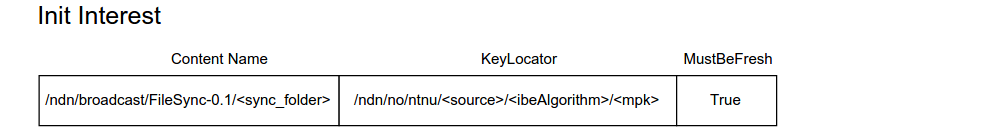
\includegraphics[width=1\textwidth]{init-sync-interest.png}
  \caption{Initialization Interest for joining a synchronization folder.}
  \label{fig:init-sync-interest}
\end{figure}

\begin{figure}[ht]
  \centering
  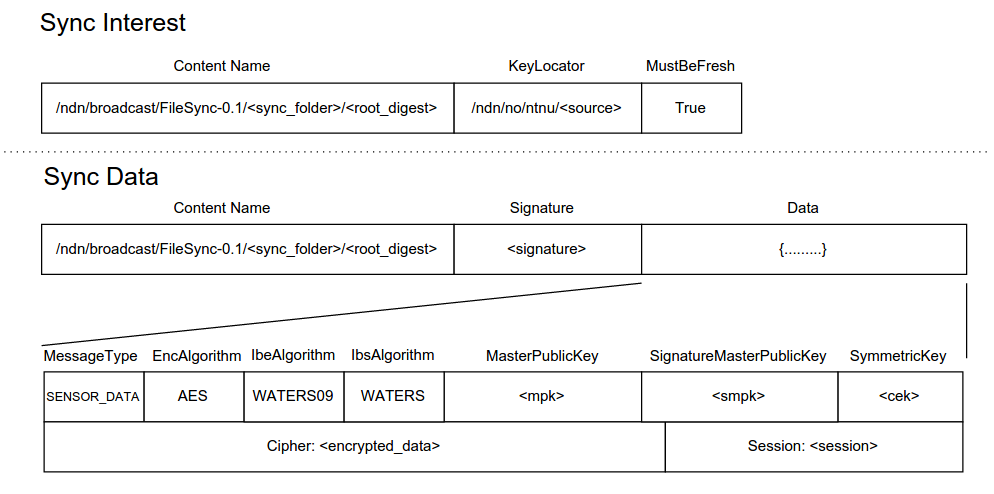
\includegraphics[width=1\textwidth]{sync-interest-data.png}
  \caption{Sync Interest and Data}
  \label{fig:sync-interest-data}
\end{figure}


\section{Sensor Application - Implementation}
Application flow explained in~\autoref{sensor-application}

Device code~\cite[device.py]{garseg15}

\gls{PKG} code~\cite[publicKeyGenerator.py]{garseg15}

Main code~\cite[application.py]{garseg15}

\subsection{Access Control}
In~\autoref{access_control} I present a possible solution for access control.
This is however not implemented in the application, because there does not exist a Python library and it is considered to be too high workload for this thesis.

\subsection{Packet Design}
Initialization packets have the structure presented in~\autoref{fig:init_interest-data}.
Initially the idea was to have the \textit{\gls{TMPK}} appended to the Content Name. 
However I experienced a problem where the Init Data never arrived at destination node. 
After some research in \texttt{ndn-cxx} documentation I found that the packets have a \texttt{MAX\_NDN\_PACKET\_SIZE} of 8800 bytes and the Init Data exceeded this limit and reached 8904 bytes.
Because the \gls{TMPK} is approximately 2\gls{KB} and was appended to the Content Name in the Interest, the Data response off course had to have the same Content Name, hence 2\gls{KB} overhead in the Name. 
The \gls{TMPK} can as easily be appended to the KeyLocator Name, hence the Data response can be 2\gls{KB} less, resulting to a 6866 bytes Init Data packet.

Sensor packets have the structure presented in~\autoref{fig:sensor_interest-data}.
\begin{description}
	\item[Init Interest] - 
  The initialization Interest seen in~\autoref{fig:init_interest-data}
  KeyLocator can be of type Name. 
  As described in the \gls{NDN} Packet Format~\cite{ndnpacketformat}, generally this field can be used to specify where to download the certificate used to sign the Interest.
  However, in our trust model we use this field to publish the requesters Name, i.e. the requesters public key. 
  This is very useful when using \gls{IBE} and \gls{IBS}.
	\item[Init Data] - 
  The Data response the the initialization Interest contains data with a structure defined in~\cite[messageBuf.proto]{garseg15} and illustrated in~\autoref{fig:init_interest-data}.
	\item[Sensor Interest] -
	As in the initialization Interest the KeyLocator field is used to define the requesters Name. ~\autoref{fig:sensor_interest-data}
	\item[Sensor Data] - 
  The Data response to the Sensor Interest uses the same structure as the initialization Data. It is illustrated in~\autoref{fig:sensor_interest-data}
\end{description}

\begin{figure}[ht]
  \centering
  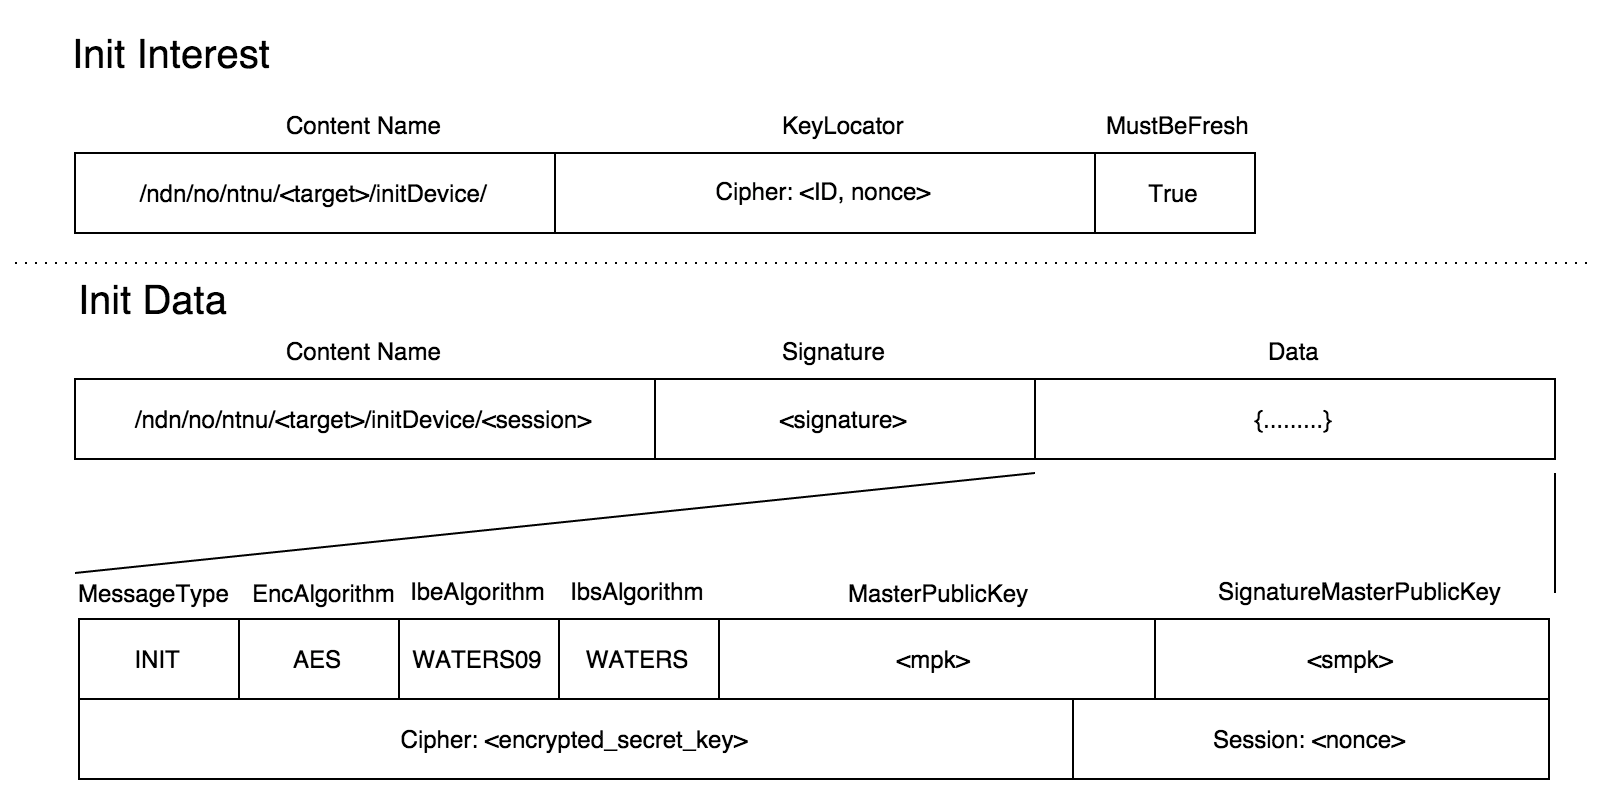
\includegraphics[width=1\textwidth]{init_interest-data.png}
  \caption{Initialization Interest and Data}
  \label{fig:init_interest-data}
\end{figure}

\begin{figure}[ht]
  \centering
  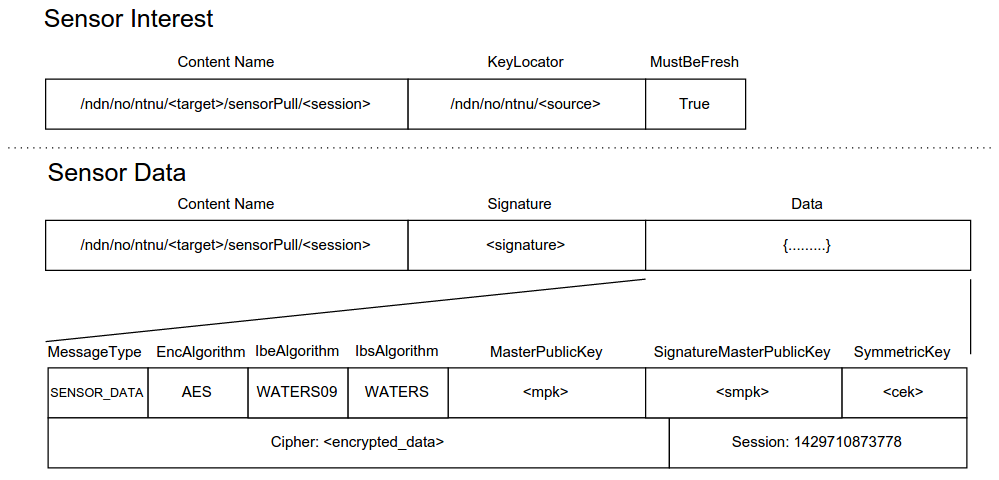
\includegraphics[width=1\textwidth]{sensor_interest-data.png}
  \caption{Sensor Interest and Data}
  \label{fig:sensor_interest-data}
\end{figure}

\section{Testing}

At first I wanted to test the application with several Raspberry Pi's to simulate a sensor network. 
However this is not possible with the Charm framework as it is not compatible with ARM processors.

\subsection{Computers}
The health sensor system is tested over several computers (see ~\autoref{tbl:target_computers} for specifications) at \gls{ntnu}.

\begin{table}[h]
  \begin{tabular}{lll}
  Computer                  & Operating System          & Processor                    \\ \hline
  Macbook Pro               & 64-bit OS X 10.10         & Intel Core i7 @ 2.0GHz       \\ %\hline
  Garsbook                  & 64-bit Ubuntu 14.04 LTS   & Intel Core i5 @ 3.0GHz       \\ %\hline
  \end{tabular}
  \caption{Computers used during tests.}
  \label{tbl:target_computers}
\end{table}

\subsection{Size}

\begin{table}[h]
  \begin{tabular}{lll}
  Data                            & Scheme          & Size (bytes)      \\ \hline
  Content Encryption Key (CEK)    & Random          & 244 bytes         \\ %\hline
  IBE Master Public Key           & Waters09        & 2014 bytes        \\ %\hline
  IBE Private Key (PK)            & Waters09        & 1164 bytes        \\ %\hline
  IBE Encrypted CEK               & Waters09        & 1472 bytes        \\ %\hline
  Encrypted PK                    & AES             & 1633 bytes        \\ %\hline
  IBS Master Public Key           & Waters          & 2360 bytes        \\ %\hline
  IBS Private Key (SPK)           & Waters          & 260 bytes         \\ %\hline
  IBS Signature                   & Waters          & 412 bytes         \\ %\hline
  Encrypted SPK                   & AES             & 437 bytes         \\ %\hline
  \end{tabular}
  \caption{Data sizes.}
  \label{tbl:size_chart}
\end{table}


\subsection{Time}
\begin{table}[h]
  \begin{tabular}{lll}
  Method                                      & Scheme          & Time (seconds)    \\ \hline
  IBE PKG Keypair generation                  & Waters09        & 0.09965           \\ %\hline
  IBE Encrypting CEK                          & Waters09        & 0.05265           \\ %\hline
  IBE Private Key (PK) generation             & Waters09        & 0.05614           \\ %\hline
  IBE Encrypting PK                           & AES             & 0.00013           \\ %\hline
  IBS PKG Keypair generation                  & Waters          & 0.09755           \\ %\hline
  IBS Private Key (SPK) generation            & Waters          & 0.00976           \\ %\hline
  IBS Sign                                    & Waters          & 0.00990           \\ %\hline
  IBS Verify                                  & Waters          & 0.00758           \\ %\hline
  Encrypting SPK                              & AES             & 0.00006           \\ %\hline
  RSA (1024-bit) keypair generation           & RSA             & 0.25427           \\ %\hline
  RSA Encryption                              & RSA             & 0.01480           \\ %\hline
  RSA Decryption                              & RSA             & 0.01472           \\ %\hline
  RSA Sign                                    & RSA             & 0.01615           \\ %\hline
  RSA Verify                                  & RSA             & 0.01572           \\ %\hline
  ECDSA keypair generation                    & ECDSA           & 0.00057           \\ %\hline
  ECDSA Sign                                  & ECDSA           & 0.00050           \\ %\hline
  ECDSA Verify                                & ECDSA           & 0.00090           \\ %\hline
  \end{tabular}
  \caption{Time table.}
  \label{tbl:time_chart}
\end{table}

\begin{table}[h]
  \begin{tabular}{lll}
  Protocol                                & Time (seconds)    \\ \hline
  Initialization                          & 0.2029            \\ %\hline
  Data Pull                               & 0.0614            \\ %\hline
  \end{tabular}
  \caption{Round Trip Time table.}
  \label{tbl:rtt_chart}
\end{table}
